\documentclass[1p]{elsarticle_modified}
%\bibliographystyle{elsarticle-num}

%\usepackage[colorlinks]{hyperref}
%\usepackage{abbrmath_seonhwa} %\Abb, \Ascr, \Acal ,\Abf, \Afrak
\usepackage{amsfonts}
\usepackage{amssymb}
\usepackage{amsmath}
\usepackage{amsthm}
\usepackage{scalefnt}
\usepackage{amsbsy}
\usepackage{kotex}
\usepackage{caption}
\usepackage{subfig}
\usepackage{color}
\usepackage{graphicx}
\usepackage{xcolor} %% white, black, red, green, blue, cyan, magenta, yellow
\usepackage{float}
\usepackage{setspace}
\usepackage{hyperref}

\usepackage{tikz}
\usetikzlibrary{arrows}

\usepackage{multirow}
\usepackage{array} % fixed length table
\usepackage{hhline}

%%%%%%%%%%%%%%%%%%%%%
\makeatletter
\renewcommand*\env@matrix[1][\arraystretch]{%
	\edef\arraystretch{#1}%
	\hskip -\arraycolsep
	\let\@ifnextchar\new@ifnextchar
	\array{*\c@MaxMatrixCols c}}
\makeatother %https://tex.stackexchange.com/questions/14071/how-can-i-increase-the-line-spacing-in-a-matrix
%%%%%%%%%%%%%%%

\usepackage[normalem]{ulem}

\newcommand{\msout}[1]{\ifmmode\text{\sout{\ensuremath{#1}}}\else\sout{#1}\fi}
%SOURCE: \msout is \stkout macro in https://tex.stackexchange.com/questions/20609/strikeout-in-math-mode

\newcommand{\cancel}[1]{
	\ifmmode
	{\color{red}\msout{#1}}
	\else
	{\color{red}\sout{#1}}
	\fi
}

\newcommand{\add}[1]{
	{\color{blue}\uwave{#1}}
}

\newcommand{\replace}[2]{
	\ifmmode
	{\color{red}\msout{#1}}{\color{blue}\uwave{#2}}
	\else
	{\color{red}\sout{#1}}{\color{blue}\uwave{#2}}
	\fi
}

\newcommand{\Sol}{\mathcal{S}} %segment
\newcommand{\D}{D} %diagram
\newcommand{\A}{\mathcal{A}} %arc


%%%%%%%%%%%%%%%%%%%%%%%%%%%%%5 test

\def\sl{\operatorname{\textup{SL}}(2,\Cbb)}
\def\psl{\operatorname{\textup{PSL}}(2,\Cbb)}
\def\quan{\mkern 1mu \triangleright \mkern 1mu}

\theoremstyle{definition}
\newtheorem{thm}{Theorem}[section]
\newtheorem{prop}[thm]{Proposition}
\newtheorem{lem}[thm]{Lemma}
\newtheorem{ques}[thm]{Question}
\newtheorem{cor}[thm]{Corollary}
\newtheorem{defn}[thm]{Definition}
\newtheorem{exam}[thm]{Example}
\newtheorem{rmk}[thm]{Remark}
\newtheorem{alg}[thm]{Algorithm}

\newcommand{\I}{\sqrt{-1}}
\begin{document}

%\begin{frontmatter}
%
%\title{Boundary parabolic representations of knots up to 8 crossings}
%
%%% Group authors per affiliation:
%\author{Yunhi Cho} 
%\address{Department of Mathematics, University of Seoul, Seoul, Korea}
%\ead{yhcho@uos.ac.kr}
%
%
%\author{Seonhwa Kim} %\fnref{s_kim}}
%\address{Center for Geometry and Physics, Institute for Basic Science, Pohang, 37673, Korea}
%\ead{ryeona17@ibs.re.kr}
%
%\author{Hyuk Kim}
%\address{Department of Mathematical Sciences, Seoul National University, Seoul 08826, Korea}
%\ead{hyukkim@snu.ac.kr}
%
%\author{Seokbeom Yoon}
%\address{Department of Mathematical Sciences, Seoul National University, Seoul, 08826,  Korea}
%\ead{sbyoon15@snu.ac.kr}
%
%\begin{abstract}
%We find all boundary parabolic representation of knots up to 8 crossings.
%
%\end{abstract}
%\begin{keyword}
%    \MSC[2010] 57M25 
%\end{keyword}
%
%\end{frontmatter}

%\linenumbers
%\tableofcontents
%
\newcommand\colored[1]{\textcolor{white}{\rule[-0.35ex]{0.8em}{1.4ex}}\kern-0.8em\color{red} #1}%
%\newcommand\colored[1]{\textcolor{white}{ #1}\kern-2.17ex	\textcolor{white}{ #1}\kern-1.81ex	\textcolor{white}{ #1}\kern-2.15ex\color{red}#1	}

{\Large $\underline{12a_{0234}~(K12a_{0234})}$}

\setlength{\tabcolsep}{10pt}
\renewcommand{\arraystretch}{1.6}
\vspace{1cm}\begin{tabular}{m{100pt}>{\centering\arraybackslash}m{274pt}}
\multirow{5}{120pt}{
	\centering
	\includegraphics[width=112pt]{../../../GIT/diagram.site/Diagrams/png/1035_12a_0234.png}\\
\ \ \ A knot diagram\footnotemark}&
\allowdisplaybreaks
\textbf{Linearized knot diagam} \\
\cline{2-2}
 &
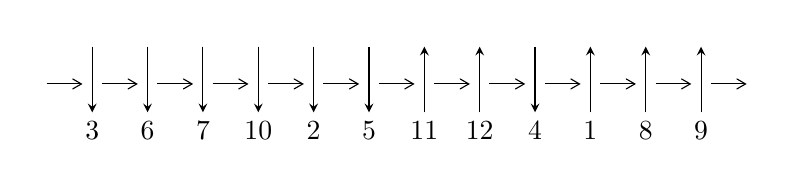
\begin{tikzpicture}[x=20pt, y=17pt]
	% nodes
	\node (C0) at (0, 0) {};
	\node (C1) at (1, 0) {};
	\node (C1U) at (1, +1) {};
	\node (C1D) at (1, -1) {3};

	\node (C2) at (2, 0) {};
	\node (C2U) at (2, +1) {};
	\node (C2D) at (2, -1) {6};

	\node (C3) at (3, 0) {};
	\node (C3U) at (3, +1) {};
	\node (C3D) at (3, -1) {7};

	\node (C4) at (4, 0) {};
	\node (C4U) at (4, +1) {};
	\node (C4D) at (4, -1) {10};

	\node (C5) at (5, 0) {};
	\node (C5U) at (5, +1) {};
	\node (C5D) at (5, -1) {2};

	\node (C6) at (6, 0) {};
	\node (C6U) at (6, +1) {};
	\node (C6D) at (6, -1) {5};

	\node (C7) at (7, 0) {};
	\node (C7U) at (7, +1) {};
	\node (C7D) at (7, -1) {11};

	\node (C8) at (8, 0) {};
	\node (C8U) at (8, +1) {};
	\node (C8D) at (8, -1) {12};

	\node (C9) at (9, 0) {};
	\node (C9U) at (9, +1) {};
	\node (C9D) at (9, -1) {4};

	\node (C10) at (10, 0) {};
	\node (C10U) at (10, +1) {};
	\node (C10D) at (10, -1) {1};

	\node (C11) at (11, 0) {};
	\node (C11U) at (11, +1) {};
	\node (C11D) at (11, -1) {8};

	\node (C12) at (12, 0) {};
	\node (C12U) at (12, +1) {};
	\node (C12D) at (12, -1) {9};
	\node (C13) at (13, 0) {};

	% arrows
	\draw[->,>={angle 60}]
	(C0) edge (C1) (C1) edge (C2) (C2) edge (C3) (C3) edge (C4) (C4) edge (C5) (C5) edge (C6) (C6) edge (C7) (C7) edge (C8) (C8) edge (C9) (C9) edge (C10) (C10) edge (C11) (C11) edge (C12) (C12) edge (C13) ;	\draw[->,>=stealth]
	(C1U) edge (C1D) (C2U) edge (C2D) (C3U) edge (C3D) (C4U) edge (C4D) (C5U) edge (C5D) (C6U) edge (C6D) (C7D) edge (C7U) (C8D) edge (C8U) (C9U) edge (C9D) (C10D) edge (C10U) (C11D) edge (C11U) (C12D) edge (C12U) ;
	\end{tikzpicture} \\
\hhline{~~} \\& 
\textbf{Solving Sequence} \\ \cline{2-2} 
 &
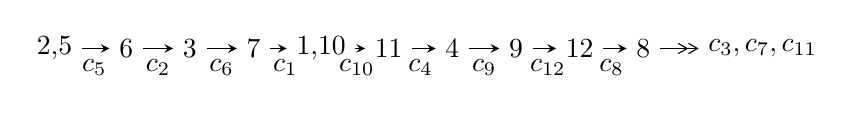
\begin{tikzpicture}[x=23pt, y=7pt]
	% node
	\node (A0) at (-1/8, 0) {2,5};
	\node (A1) at (1, 0) {6};
	\node (A2) at (2, 0) {3};
	\node (A3) at (3, 0) {7};
	\node (A4) at (65/16, 0) {1,10};
	\node (A5) at (41/8, 0) {11};
	\node (A6) at (49/8, 0) {4};
	\node (A7) at (57/8, 0) {9};
	\node (A8) at (65/8, 0) {12};
	\node (A9) at (73/8, 0) {8};
	\node (C1) at (1/2, -1) {$c_{5}$};
	\node (C2) at (3/2, -1) {$c_{2}$};
	\node (C3) at (5/2, -1) {$c_{6}$};
	\node (C4) at (7/2, -1) {$c_{1}$};
	\node (C5) at (37/8, -1) {$c_{10}$};
	\node (C6) at (45/8, -1) {$c_{4}$};
	\node (C7) at (53/8, -1) {$c_{9}$};
	\node (C8) at (61/8, -1) {$c_{12}$};
	\node (C9) at (69/8, -1) {$c_{8}$};
	\node (A10) at (11, 0) {$c_{3},c_{7},c_{11}$};

	% edge
	\draw[->,>=stealth]	
	(A0) edge (A1) (A1) edge (A2) (A2) edge (A3) (A3) edge (A4) (A4) edge (A5) (A5) edge (A6) (A6) edge (A7) (A7) edge (A8) (A8) edge (A9) ;
	\draw[->>,>={angle 60}]	
	(A9) edge (A10);
\end{tikzpicture} \\ 

\end{tabular} \\

\footnotetext{
The image of knot diagram is generated by the software ``\textbf{Draw programme}" developed by Andrew Bartholomew(\url{http://www.layer8.co.uk/maths/draw/index.htm\#Running-draw}), where we modified some parts for our purpose(\url{https://github.com/CATsTAILs/LinksPainter}).
}\phantom \\ \newline 
\centering \textbf{Ideals for irreducible components\footnotemark of $X_{\text{par}}$} 
 
\begin{align*}
I^u_{1}&=\langle 
u^{74}+u^{73}+\cdots+b- u,\;-10 u^{74}-43 u^{73}+\cdots+2 a-15,\;u^{75}+4 u^{74}+\cdots+4 u+1\rangle \\
I^u_{2}&=\langle 
b,\;a^2- a u- u^2+a+2 u-1,\;u^3- u^2+1\rangle \\
I^u_{3}&=\langle 
b-1,\;a-2,\;u-1\rangle \\
\\
\end{align*}
\raggedright * 3 irreducible components of $\dim_{\mathbb{C}}=0$, with total 82 representations.\\
\footnotetext{All coefficients of polynomials are rational numbers. But the coefficients are sometimes approximated in decimal forms when there is not enough margin.}
\newpage
\renewcommand{\arraystretch}{1}
\centering \section*{I. $I^u_{1}= \langle u^{74}+u^{73}+\cdots+b- u,\;-10 u^{74}-43 u^{73}+\cdots+2 a-15,\;u^{75}+4 u^{74}+\cdots+4 u+1 \rangle$}
\flushleft \textbf{(i) Arc colorings}\\
\begin{tabular}{m{7pt} m{180pt} m{7pt} m{180pt} }
\flushright $a_{2}=$&$\begin{pmatrix}0\\u\end{pmatrix}$ \\
\flushright $a_{5}=$&$\begin{pmatrix}1\\0\end{pmatrix}$ \\
\flushright $a_{6}=$&$\begin{pmatrix}1\\u^2\end{pmatrix}$ \\
\flushright $a_{3}=$&$\begin{pmatrix}- u\\- u^3+u\end{pmatrix}$ \\
\flushright $a_{7}=$&$\begin{pmatrix}- u^2+1\\u^2\end{pmatrix}$ \\
\flushright $a_{1}=$&$\begin{pmatrix}u^3\\u^5- u^3+u\end{pmatrix}$ \\
\flushright $a_{10}=$&$\begin{pmatrix}5 u^{74}+\frac{43}{2} u^{73}+\cdots+\frac{39}{2} u+\frac{15}{2}\\- u^{74}- u^{73}+\cdots+4 u^2+u\end{pmatrix}$ \\
\flushright $a_{11}=$&$\begin{pmatrix}\frac{5}{2} u^{74}+11 u^{73}+\cdots+\frac{13}{2} u+3\\\frac{1}{2} u^{74}+\frac{5}{2} u^{73}+\cdots+4 u+1\end{pmatrix}$ \\
\flushright $a_{4}=$&$\begin{pmatrix}u^7-2 u^5+2 u^3-2 u\\- u^7+u^5-2 u^3+u\end{pmatrix}$ \\
\flushright $a_{9}=$&$\begin{pmatrix}2 u^{74}+\frac{5}{2} u^{73}+\cdots-\frac{19}{2} u-\frac{5}{2}\\6 u^{74}+23 u^{73}+\cdots+27 u+8\end{pmatrix}$ \\
\flushright $a_{12}=$&$\begin{pmatrix}-\frac{1}{2} u^{73}- u^{72}+\cdots+\frac{5}{2} u+\frac{1}{2}\\u^{26}-4 u^{24}+\cdots-4 u^3-3 u^2\end{pmatrix}$ \\
\flushright $a_{8}=$&$\begin{pmatrix}\frac{1}{2} u^{74}+u^{73}+\cdots-\frac{13}{2} u^2-\frac{7}{2} u\\\frac{1}{2} u^{74}+\frac{5}{2} u^{73}+\cdots+4 u+1\end{pmatrix}$\\&\end{tabular}
\flushleft \textbf{(ii) Obstruction class $= -1$}\\~\\
\flushleft \textbf{(iii) Cusp Shapes $= -31 u^{74}-\frac{187}{2} u^{73}+\cdots-\frac{159}{2} u-23$}\\~\\
\newpage\renewcommand{\arraystretch}{1}
\flushleft \textbf{(iv) u-Polynomials at the component}\newline \\
\begin{tabular}{m{50pt}|m{274pt}}
Crossings & \hspace{64pt}u-Polynomials at each crossing \\
\hline $$\begin{aligned}c_{1},c_{6}\end{aligned}$$&$\begin{aligned}
&u^{75}+24 u^{74}+\cdots-16 u+1
\end{aligned}$\\
\hline $$\begin{aligned}c_{2},c_{5}\end{aligned}$$&$\begin{aligned}
&u^{75}+4 u^{74}+\cdots+4 u+1
\end{aligned}$\\
\hline $$\begin{aligned}c_{3}\end{aligned}$$&$\begin{aligned}
&u^{75}-2 u^{74}+\cdots-2768 u+1009
\end{aligned}$\\
\hline $$\begin{aligned}c_{4},c_{9}\end{aligned}$$&$\begin{aligned}
&u^{75}-2 u^{74}+\cdots+32 u-64
\end{aligned}$\\
\hline $$\begin{aligned}c_{7},c_{8},c_{11}\\c_{12}\end{aligned}$$&$\begin{aligned}
&u^{75}-3 u^{74}+\cdots-7 u-1
\end{aligned}$\\
\hline $$\begin{aligned}c_{10}\end{aligned}$$&$\begin{aligned}
&u^{75}+21 u^{74}+\cdots-4045 u+239
\end{aligned}$\\
\hline
\end{tabular}\\~\\
\newpage\renewcommand{\arraystretch}{1}
\flushleft \textbf{(v) Riley Polynomials at the component}\newline \\
\begin{tabular}{m{50pt}|m{274pt}}
Crossings & \hspace{64pt}Riley Polynomials at each crossing \\
\hline $$\begin{aligned}c_{1},c_{6}\end{aligned}$$&$\begin{aligned}
&y^{75}+56 y^{74}+\cdots+160 y-1
\end{aligned}$\\
\hline $$\begin{aligned}c_{2},c_{5}\end{aligned}$$&$\begin{aligned}
&y^{75}-24 y^{74}+\cdots-16 y-1
\end{aligned}$\\
\hline $$\begin{aligned}c_{3}\end{aligned}$$&$\begin{aligned}
&y^{75}-4 y^{74}+\cdots-1197196 y-1018081
\end{aligned}$\\
\hline $$\begin{aligned}c_{4},c_{9}\end{aligned}$$&$\begin{aligned}
&y^{75}-34 y^{74}+\cdots+82944 y-4096
\end{aligned}$\\
\hline $$\begin{aligned}c_{7},c_{8},c_{11}\\c_{12}\end{aligned}$$&$\begin{aligned}
&y^{75}-87 y^{74}+\cdots+53 y-1
\end{aligned}$\\
\hline $$\begin{aligned}c_{10}\end{aligned}$$&$\begin{aligned}
&y^{75}-3 y^{74}+\cdots+27550093 y-57121
\end{aligned}$\\
\hline
\end{tabular}\\~\\
\newpage\flushleft \textbf{(vi) Complex Volumes and Cusp Shapes}
$$\begin{array}{c|c|c}  
\text{Solutions to }I^u_{1}& \I (\text{vol} + \sqrt{-1}CS) & \text{Cusp shape}\\
 \hline 
\begin{aligned}
u &= -0.711207 + 0.731942 I \\
a &= \phantom{-}0.073783 + 0.958389 I \\
b &= -0.923873 - 0.439880 I\end{aligned}
 & \phantom{-}3.44957 + 0.11709 I & \phantom{-0.000000 } 0 \\ \hline\begin{aligned}
u &= -0.711207 - 0.731942 I \\
a &= \phantom{-}0.073783 - 0.958389 I \\
b &= -0.923873 + 0.439880 I\end{aligned}
 & \phantom{-}3.44957 - 0.11709 I & \phantom{-0.000000 } 0 \\ \hline\begin{aligned}
u &= -1.016490 + 0.108693 I \\
a &= \phantom{-}0.1180520 - 0.0250300 I \\
b &= -0.383356 - 1.026800 I\end{aligned}
 & \phantom{-}5.05953 + 3.13748 I & \phantom{-0.000000 } 0 \\ \hline\begin{aligned}
u &= -1.016490 - 0.108693 I \\
a &= \phantom{-}0.1180520 + 0.0250300 I \\
b &= -0.383356 + 1.026800 I\end{aligned}
 & \phantom{-}5.05953 - 3.13748 I & \phantom{-0.000000 } 0 \\ \hline\begin{aligned}
u &= -0.660509 + 0.785762 I \\
a &= -0.663561 - 0.985879 I \\
b &= \phantom{-}1.107580 + 0.521055 I\end{aligned}
 & -0.12076 - 2.74550 I & \phantom{-0.000000 } 0 \\ \hline\begin{aligned}
u &= -0.660509 - 0.785762 I \\
a &= -0.663561 + 0.985879 I \\
b &= \phantom{-}1.107580 - 0.521055 I\end{aligned}
 & -0.12076 + 2.74550 I & \phantom{-0.000000 } 0 \\ \hline\begin{aligned}
u &= -0.965638 + 0.051778 I \\
a &= -0.0394728 + 0.0390828 I \\
b &= \phantom{-}0.172922 + 0.877447 I\end{aligned}
 & -1.86895 + 1.44234 I & \phantom{-0.000000 } 0 \\ \hline\begin{aligned}
u &= -0.965638 - 0.051778 I \\
a &= -0.0394728 - 0.0390828 I \\
b &= \phantom{-}0.172922 - 0.877447 I\end{aligned}
 & -1.86895 - 1.44234 I & \phantom{-0.000000 } 0 \\ \hline\begin{aligned}
u &= \phantom{-}0.722226 + 0.744545 I \\
a &= \phantom{-}0.18997 + 1.79205 I \\
b &= -0.477443 - 0.900673 I\end{aligned}
 & \phantom{-}3.49030 + 0.98913 I & \phantom{-0.000000 } 0 \\ \hline\begin{aligned}
u &= \phantom{-}0.722226 - 0.744545 I \\
a &= \phantom{-}0.18997 - 1.79205 I \\
b &= -0.477443 + 0.900673 I\end{aligned}
 & \phantom{-}3.49030 - 0.98913 I & \phantom{-0.000000 } 0\\
 \hline 
 \end{array}$$\newpage$$\begin{array}{c|c|c}  
\text{Solutions to }I^u_{1}& \I (\text{vol} + \sqrt{-1}CS) & \text{Cusp shape}\\
 \hline 
\begin{aligned}
u &= \phantom{-}0.697965 + 0.783588 I \\
a &= -0.35474 - 1.96967 I \\
b &= \phantom{-}0.569105 + 1.003110 I\end{aligned}
 & \phantom{-}11.08350 + 2.94021 I & \phantom{-0.000000 } 0 \\ \hline\begin{aligned}
u &= \phantom{-}0.697965 - 0.783588 I \\
a &= -0.35474 + 1.96967 I \\
b &= \phantom{-}0.569105 - 1.003110 I\end{aligned}
 & \phantom{-}11.08350 - 2.94021 I & \phantom{-0.000000 } 0 \\ \hline\begin{aligned}
u &= \phantom{-}0.785691 + 0.697977 I \\
a &= \phantom{-}0.09437 - 1.44165 I \\
b &= \phantom{-}0.324972 + 0.756336 I\end{aligned}
 & \phantom{-}2.20022 - 1.98773 I & \phantom{-0.000000 } 0 \\ \hline\begin{aligned}
u &= \phantom{-}0.785691 - 0.697977 I \\
a &= \phantom{-}0.09437 + 1.44165 I \\
b &= \phantom{-}0.324972 - 0.756336 I\end{aligned}
 & \phantom{-}2.20022 + 1.98773 I & \phantom{-0.000000 } 0 \\ \hline\begin{aligned}
u &= -0.671002 + 0.820090 I \\
a &= \phantom{-}0.83769 + 1.20399 I \\
b &= -1.140810 - 0.631940 I\end{aligned}
 & \phantom{-}1.38833 - 6.65529 I & \phantom{-0.000000 } 0 \\ \hline\begin{aligned}
u &= -0.671002 - 0.820090 I \\
a &= \phantom{-}0.83769 - 1.20399 I \\
b &= -1.140810 + 0.631940 I\end{aligned}
 & \phantom{-}1.38833 + 6.65529 I & \phantom{-0.000000 } 0 \\ \hline\begin{aligned}
u &= \phantom{-}1.06726\phantom{ +0.000000I} \\
a &= \phantom{-}1.51914\phantom{ +0.000000I} \\
b &= \phantom{-}1.24765\phantom{ +0.000000I}\end{aligned}
 & -1.46846\phantom{ +0.000000I} & \phantom{-0.000000 } 0 \\ \hline\begin{aligned}
u &= \phantom{-}1.063370 + 0.091921 I \\
a &= -1.48543 + 0.57951 I \\
b &= -1.204920 - 0.351467 I\end{aligned}
 & -6.19357 - 2.44894 I & \phantom{-0.000000 } 0 \\ \hline\begin{aligned}
u &= \phantom{-}1.063370 - 0.091921 I \\
a &= -1.48543 - 0.57951 I \\
b &= -1.204920 + 0.351467 I\end{aligned}
 & -6.19357 + 2.44894 I & \phantom{-0.000000 } 0 \\ \hline\begin{aligned}
u &= -0.766146 + 0.749616 I \\
a &= \phantom{-}0.30396 - 1.44485 I \\
b &= \phantom{-}0.764353 + 0.496302 I\end{aligned}
 & \phantom{-}12.27310 + 1.21172 I & \phantom{-0.000000 } 0\\
 \hline 
 \end{array}$$\newpage$$\begin{array}{c|c|c}  
\text{Solutions to }I^u_{1}& \I (\text{vol} + \sqrt{-1}CS) & \text{Cusp shape}\\
 \hline 
\begin{aligned}
u &= -0.766146 - 0.749616 I \\
a &= \phantom{-}0.30396 + 1.44485 I \\
b &= \phantom{-}0.764353 - 0.496302 I\end{aligned}
 & \phantom{-}12.27310 - 1.21172 I & \phantom{-0.000000 } 0 \\ \hline\begin{aligned}
u &= \phantom{-}0.908509 + 0.580630 I \\
a &= -0.94613 + 1.40143 I \\
b &= -0.107565 - 0.998481 I\end{aligned}
 & \phantom{-}7.57381 - 2.23045 I & \phantom{-0.000000 } 0 \\ \hline\begin{aligned}
u &= \phantom{-}0.908509 - 0.580630 I \\
a &= -0.94613 - 1.40143 I \\
b &= -0.107565 + 0.998481 I\end{aligned}
 & \phantom{-}7.57381 + 2.23045 I & \phantom{-0.000000 } 0 \\ \hline\begin{aligned}
u &= \phantom{-}1.072730 + 0.131160 I \\
a &= \phantom{-}1.38515 - 0.78395 I \\
b &= \phantom{-}1.210390 + 0.505142 I\end{aligned}
 & -5.10143 - 6.45888 I & \phantom{-0.000000 } 0 \\ \hline\begin{aligned}
u &= \phantom{-}1.072730 - 0.131160 I \\
a &= \phantom{-}1.38515 + 0.78395 I \\
b &= \phantom{-}1.210390 - 0.505142 I\end{aligned}
 & -5.10143 + 6.45888 I & \phantom{-0.000000 } 0 \\ \hline\begin{aligned}
u &= -0.682230 + 0.841524 I \\
a &= -0.94322 - 1.37024 I \\
b &= \phantom{-}1.151480 + 0.720103 I\end{aligned}
 & \phantom{-}9.20789 - 9.23314 I & \phantom{-0.000000 } 0 \\ \hline\begin{aligned}
u &= -0.682230 - 0.841524 I \\
a &= -0.94322 + 1.37024 I \\
b &= \phantom{-}1.151480 - 0.720103 I\end{aligned}
 & \phantom{-}9.20789 + 9.23314 I & \phantom{-0.000000 } 0 \\ \hline\begin{aligned}
u &= -0.993937 + 0.434871 I \\
a &= \phantom{-}0.133903 - 0.616443 I \\
b &= -1.174540 - 0.467698 I\end{aligned}
 & \phantom{-}4.04103 - 2.59869 I & \phantom{-0.000000 } 0 \\ \hline\begin{aligned}
u &= -0.993937 - 0.434871 I \\
a &= \phantom{-}0.133903 + 0.616443 I \\
b &= -1.174540 + 0.467698 I\end{aligned}
 & \phantom{-}4.04103 + 2.59869 I & \phantom{-0.000000 } 0 \\ \hline\begin{aligned}
u &= -0.971580 + 0.501941 I \\
a &= \phantom{-}0.063789 + 0.774786 I \\
b &= \phantom{-}1.174790 + 0.276036 I\end{aligned}
 & -2.94814 - 0.18097 I & \phantom{-0.000000 } 0\\
 \hline 
 \end{array}$$\newpage$$\begin{array}{c|c|c}  
\text{Solutions to }I^u_{1}& \I (\text{vol} + \sqrt{-1}CS) & \text{Cusp shape}\\
 \hline 
\begin{aligned}
u &= -0.971580 - 0.501941 I \\
a &= \phantom{-}0.063789 - 0.774786 I \\
b &= \phantom{-}1.174790 - 0.276036 I\end{aligned}
 & -2.94814 + 0.18097 I & \phantom{-0.000000 } 0 \\ \hline\begin{aligned}
u &= \phantom{-}1.081740 + 0.163201 I \\
a &= -1.30157 + 0.93027 I \\
b &= -1.210650 - 0.632851 I\end{aligned}
 & \phantom{-}2.40082 - 9.12230 I & \phantom{-0.000000 } 0 \\ \hline\begin{aligned}
u &= \phantom{-}1.081740 - 0.163201 I \\
a &= -1.30157 - 0.93027 I \\
b &= -1.210650 + 0.632851 I\end{aligned}
 & \phantom{-}2.40082 + 9.12230 I & \phantom{-0.000000 } 0 \\ \hline\begin{aligned}
u &= \phantom{-}0.888282\phantom{ +0.000000I} \\
a &= -3.24544\phantom{ +0.000000I} \\
b &= -0.629954\phantom{ +0.000000I}\end{aligned}
 & \phantom{-}7.31928\phantom{ +0.000000I} & -10.6220\phantom{ +0.000000I} \\ \hline\begin{aligned}
u &= -0.982759 + 0.562329 I \\
a &= -0.216181 - 1.041120 I \\
b &= -1.209770 - 0.100303 I\end{aligned}
 & -3.43339 + 3.68758 I & \phantom{-0.000000 } 0 \\ \hline\begin{aligned}
u &= -0.982759 - 0.562329 I \\
a &= -0.216181 + 1.041120 I \\
b &= -1.209770 + 0.100303 I\end{aligned}
 & -3.43339 - 3.68758 I & \phantom{-0.000000 } 0 \\ \hline\begin{aligned}
u &= -0.499811 + 0.691420 I \\
a &= \phantom{-}0.744111 - 0.062254 I \\
b &= -1.178410 - 0.102990 I\end{aligned}
 & \phantom{-}3.70237 - 1.18565 I & \phantom{-}0.324301 + 0.368937 I \\ \hline\begin{aligned}
u &= -0.499811 - 0.691420 I \\
a &= \phantom{-}0.744111 + 0.062254 I \\
b &= -1.178410 + 0.102990 I\end{aligned}
 & \phantom{-}3.70237 + 1.18565 I & \phantom{-}0.324301 - 0.368937 I \\ \hline\begin{aligned}
u &= \phantom{-}0.836198 + 0.792398 I \\
a &= \phantom{-}0.716749 + 1.015140 I \\
b &= -0.683410 - 0.394873 I\end{aligned}
 & \phantom{-}4.26586 - 3.75101 I & \phantom{-0.000000 } 0 \\ \hline\begin{aligned}
u &= \phantom{-}0.836198 - 0.792398 I \\
a &= \phantom{-}0.716749 - 1.015140 I \\
b &= -0.683410 + 0.394873 I\end{aligned}
 & \phantom{-}4.26586 + 3.75101 I & \phantom{-0.000000 } 0\\
 \hline 
 \end{array}$$\newpage$$\begin{array}{c|c|c}  
\text{Solutions to }I^u_{1}& \I (\text{vol} + \sqrt{-1}CS) & \text{Cusp shape}\\
 \hline 
\begin{aligned}
u &= \phantom{-}0.937039 + 0.676923 I \\
a &= \phantom{-}1.012900 - 0.915123 I \\
b &= -0.211047 + 0.866238 I\end{aligned}
 & \phantom{-}1.72641 - 3.30860 I & \phantom{-0.000000 } 0 \\ \hline\begin{aligned}
u &= \phantom{-}0.937039 - 0.676923 I \\
a &= \phantom{-}1.012900 + 0.915123 I \\
b &= -0.211047 - 0.866238 I\end{aligned}
 & \phantom{-}1.72641 + 3.30860 I & \phantom{-0.000000 } 0 \\ \hline\begin{aligned}
u &= \phantom{-}0.826326 + 0.828687 I \\
a &= -1.00165 - 1.24716 I \\
b &= \phantom{-}0.907683 + 0.488606 I\end{aligned}
 & \phantom{-}11.80470 - 5.23133 I & \phantom{-0.000000 } 0 \\ \hline\begin{aligned}
u &= \phantom{-}0.826326 - 0.828687 I \\
a &= -1.00165 + 1.24716 I \\
b &= \phantom{-}0.907683 - 0.488606 I\end{aligned}
 & \phantom{-}11.80470 + 5.23133 I & \phantom{-0.000000 } 0 \\ \hline\begin{aligned}
u &= -1.010410 + 0.619026 I \\
a &= \phantom{-}0.27560 + 1.47068 I \\
b &= \phantom{-}1.274680 - 0.127579 I\end{aligned}
 & \phantom{-}2.28478 + 6.17362 I & \phantom{-0.000000 } 0 \\ \hline\begin{aligned}
u &= -1.010410 - 0.619026 I \\
a &= \phantom{-}0.27560 - 1.47068 I \\
b &= \phantom{-}1.274680 + 0.127579 I\end{aligned}
 & \phantom{-}2.28478 - 6.17362 I & \phantom{-0.000000 } 0 \\ \hline\begin{aligned}
u &= -0.952521 + 0.709229 I \\
a &= -1.25985 - 2.13172 I \\
b &= -0.819855 + 0.405800 I\end{aligned}
 & \phantom{-}11.70100 + 4.33992 I & \phantom{-0.000000 } 0 \\ \hline\begin{aligned}
u &= -0.952521 - 0.709229 I \\
a &= -1.25985 + 2.13172 I \\
b &= -0.819855 - 0.405800 I\end{aligned}
 & \phantom{-}11.70100 - 4.33992 I & \phantom{-0.000000 } 0 \\ \hline\begin{aligned}
u &= \phantom{-}0.914778 + 0.769195 I \\
a &= -1.046570 - 0.021063 I \\
b &= \phantom{-}0.622847 - 0.319420 I\end{aligned}
 & \phantom{-}4.02488 - 2.11438 I & \phantom{-0.000000 } 0 \\ \hline\begin{aligned}
u &= \phantom{-}0.914778 - 0.769195 I \\
a &= -1.046570 + 0.021063 I \\
b &= \phantom{-}0.622847 + 0.319420 I\end{aligned}
 & \phantom{-}4.02488 + 2.11438 I & \phantom{-0.000000 } 0\\
 \hline 
 \end{array}$$\newpage$$\begin{array}{c|c|c}  
\text{Solutions to }I^u_{1}& \I (\text{vol} + \sqrt{-1}CS) & \text{Cusp shape}\\
 \hline 
\begin{aligned}
u &= -0.982465 + 0.687726 I \\
a &= \phantom{-}0.78718 + 1.95441 I \\
b &= \phantom{-}1.032380 - 0.389930 I\end{aligned}
 & \phantom{-}2.62497 + 5.32088 I & \phantom{-0.000000 } 0 \\ \hline\begin{aligned}
u &= -0.982465 - 0.687726 I \\
a &= \phantom{-}0.78718 - 1.95441 I \\
b &= \phantom{-}1.032380 + 0.389930 I\end{aligned}
 & \phantom{-}2.62497 - 5.32088 I & \phantom{-0.000000 } 0 \\ \hline\begin{aligned}
u &= \phantom{-}0.976735 + 0.698504 I \\
a &= -1.30467 + 0.82935 I \\
b &= \phantom{-}0.428493 - 0.975607 I\end{aligned}
 & \phantom{-}2.71841 - 6.49505 I & \phantom{-0.000000 } 0 \\ \hline\begin{aligned}
u &= \phantom{-}0.976735 - 0.698504 I \\
a &= -1.30467 - 0.82935 I \\
b &= \phantom{-}0.428493 + 0.975607 I\end{aligned}
 & \phantom{-}2.71841 + 6.49505 I & \phantom{-0.000000 } 0 \\ \hline\begin{aligned}
u &= \phantom{-}0.999165 + 0.711748 I \\
a &= \phantom{-}1.48010 - 0.81442 I \\
b &= -0.557335 + 1.061150 I\end{aligned}
 & \phantom{-}10.17200 - 8.59556 I & \phantom{-0.000000 } 0 \\ \hline\begin{aligned}
u &= \phantom{-}0.999165 - 0.711748 I \\
a &= \phantom{-}1.48010 + 0.81442 I \\
b &= -0.557335 - 1.061150 I\end{aligned}
 & \phantom{-}10.17200 + 8.59556 I & \phantom{-0.000000 } 0 \\ \hline\begin{aligned}
u &= \phantom{-}0.940369 + 0.791453 I \\
a &= \phantom{-}1.42868 + 0.04316 I \\
b &= -0.886134 + 0.434484 I\end{aligned}
 & \phantom{-}11.45350 - 0.81358 I & \phantom{-0.000000 } 0 \\ \hline\begin{aligned}
u &= \phantom{-}0.940369 - 0.791453 I \\
a &= \phantom{-}1.42868 - 0.04316 I \\
b &= -0.886134 - 0.434484 I\end{aligned}
 & \phantom{-}11.45350 + 0.81358 I & \phantom{-0.000000 } 0 \\ \hline\begin{aligned}
u &= -1.015930 + 0.701587 I \\
a &= -0.47859 - 2.18042 I \\
b &= -1.177240 + 0.537485 I\end{aligned}
 & -1.18776 + 8.36921 I & \phantom{-0.000000 } 0 \\ \hline\begin{aligned}
u &= -1.015930 - 0.701587 I \\
a &= -0.47859 + 2.18042 I \\
b &= -1.177240 - 0.537485 I\end{aligned}
 & -1.18776 - 8.36921 I & \phantom{-0.000000 } 0\\
 \hline 
 \end{array}$$\newpage$$\begin{array}{c|c|c}  
\text{Solutions to }I^u_{1}& \I (\text{vol} + \sqrt{-1}CS) & \text{Cusp shape}\\
 \hline 
\begin{aligned}
u &= -1.023410 + 0.718352 I \\
a &= \phantom{-}0.43055 + 2.34903 I \\
b &= \phantom{-}1.186660 - 0.649196 I\end{aligned}
 & \phantom{-}0.31813 + 12.42890 I & \phantom{-0.000000 } 0 \\ \hline\begin{aligned}
u &= -1.023410 - 0.718352 I \\
a &= \phantom{-}0.43055 - 2.34903 I \\
b &= \phantom{-}1.186660 + 0.649196 I\end{aligned}
 & \phantom{-}0.31813 - 12.42890 I & \phantom{-0.000000 } 0 \\ \hline\begin{aligned}
u &= -1.026990 + 0.731679 I \\
a &= -0.40791 - 2.47441 I \\
b &= -1.181080 + 0.737477 I\end{aligned}
 & \phantom{-}8.1534 + 15.1124 I & \phantom{-0.000000 } 0 \\ \hline\begin{aligned}
u &= -1.026990 - 0.731679 I \\
a &= -0.40791 + 2.47441 I \\
b &= -1.181080 - 0.737477 I\end{aligned}
 & \phantom{-}8.1534 - 15.1124 I & \phantom{-0.000000 } 0 \\ \hline\begin{aligned}
u &= -0.170137 + 0.694294 I \\
a &= -0.93682 + 1.35426 I \\
b &= \phantom{-}1.121250 - 0.579634 I\end{aligned}
 & \phantom{-}6.51786 + 6.48932 I & \phantom{-}3.20143 - 4.96610 I \\ \hline\begin{aligned}
u &= -0.170137 - 0.694294 I \\
a &= -0.93682 - 1.35426 I \\
b &= \phantom{-}1.121250 + 0.579634 I\end{aligned}
 & \phantom{-}6.51786 - 6.48932 I & \phantom{-}3.20143 + 4.96610 I \\ \hline\begin{aligned}
u &= -0.222380 + 0.645831 I \\
a &= \phantom{-}0.772263 - 1.148320 I \\
b &= -1.070320 + 0.435701 I\end{aligned}
 & -0.91107 + 4.17004 I & -0.03505 - 6.87095 I \\ \hline\begin{aligned}
u &= -0.222380 - 0.645831 I \\
a &= \phantom{-}0.772263 + 1.148320 I \\
b &= -1.070320 - 0.435701 I\end{aligned}
 & -0.91107 - 4.17004 I & -0.03505 + 6.87095 I \\ \hline\begin{aligned}
u &= -0.330794 + 0.589043 I \\
a &= -0.558254 + 0.771750 I \\
b &= \phantom{-}1.021100 - 0.213253 I\end{aligned}
 & -1.84200 + 0.63905 I & -3.61059 - 0.19351 I \\ \hline\begin{aligned}
u &= -0.330794 - 0.589043 I \\
a &= -0.558254 - 0.771750 I \\
b &= \phantom{-}1.021100 + 0.213253 I\end{aligned}
 & -1.84200 - 0.63905 I & -3.61059 + 0.19351 I\\
 \hline 
 \end{array}$$\newpage$$\begin{array}{c|c|c}  
\text{Solutions to }I^u_{1}& \I (\text{vol} + \sqrt{-1}CS) & \text{Cusp shape}\\
 \hline 
\begin{aligned}
u &= -0.671696\phantom{ +0.000000I} \\
a &= \phantom{-}0.135845\phantom{ +0.000000I} \\
b &= \phantom{-}0.375009\phantom{ +0.000000I}\end{aligned}
 & -0.909794\phantom{ +0.000000I} & -11.9330\phantom{ +0.000000I} \\ \hline\begin{aligned}
u &= \phantom{-}0.185398 + 0.482510 I \\
a &= -0.25875 + 2.28529 I \\
b &= \phantom{-}0.376277 - 0.783708 I\end{aligned}
 & \phantom{-}8.74623 - 1.35684 I & \phantom{-}6.78331 + 0.85499 I \\ \hline\begin{aligned}
u &= \phantom{-}0.185398 - 0.482510 I \\
a &= -0.25875 - 2.28529 I \\
b &= \phantom{-}0.376277 + 0.783708 I\end{aligned}
 & \phantom{-}8.74623 + 1.35684 I & \phantom{-}6.78331 - 0.85499 I \\ \hline\begin{aligned}
u &= \phantom{-}0.066176 + 0.284258 I \\
a &= -0.35019 - 2.23595 I \\
b &= -0.345577 + 0.468199 I\end{aligned}
 & \phantom{-}1.171050 - 0.405728 I & \phantom{-}7.00634 + 1.53169 I \\ \hline\begin{aligned}
u &= \phantom{-}0.066176 - 0.284258 I \\
a &= -0.35019 + 2.23595 I \\
b &= -0.345577 - 0.468199 I\end{aligned}
 & \phantom{-}1.171050 + 0.405728 I & \phantom{-}7.00634 - 1.53169 I\\
 \hline 
 \end{array}$$\newpage\newpage\renewcommand{\arraystretch}{1}
\centering \section*{II. $I^u_{2}= \langle b,\;a^2- a u- u^2+a+2 u-1,\;u^3- u^2+1 \rangle$}
\flushleft \textbf{(i) Arc colorings}\\
\begin{tabular}{m{7pt} m{180pt} m{7pt} m{180pt} }
\flushright $a_{2}=$&$\begin{pmatrix}0\\u\end{pmatrix}$ \\
\flushright $a_{5}=$&$\begin{pmatrix}1\\0\end{pmatrix}$ \\
\flushright $a_{6}=$&$\begin{pmatrix}1\\u^2\end{pmatrix}$ \\
\flushright $a_{3}=$&$\begin{pmatrix}- u\\- u^2+u+1\end{pmatrix}$ \\
\flushright $a_{7}=$&$\begin{pmatrix}- u^2+1\\u^2\end{pmatrix}$ \\
\flushright $a_{1}=$&$\begin{pmatrix}u^2-1\\- u^2\end{pmatrix}$ \\
\flushright $a_{10}=$&$\begin{pmatrix}a\\0\end{pmatrix}$ \\
\flushright $a_{11}=$&$\begin{pmatrix}- a u\\- u^2 a+a u+a\end{pmatrix}$ \\
\flushright $a_{4}=$&$\begin{pmatrix}1\\0\end{pmatrix}$ \\
\flushright $a_{9}=$&$\begin{pmatrix}a\\0\end{pmatrix}$ \\
\flushright $a_{12}=$&$\begin{pmatrix}u^2- a- u\\- u^2\end{pmatrix}$ \\
\flushright $a_{8}=$&$\begin{pmatrix}a u- u+1\\u^2 a- a u- a\end{pmatrix}$\\&\end{tabular}
\flushleft \textbf{(ii) Obstruction class $= 1$}\\~\\
\flushleft \textbf{(iii) Cusp Shapes $= - u^2 a+3 u^2- a+1$}\\~\\
\newpage\renewcommand{\arraystretch}{1}
\flushleft \textbf{(iv) u-Polynomials at the component}\newline \\
\begin{tabular}{m{50pt}|m{274pt}}
Crossings & \hspace{64pt}u-Polynomials at each crossing \\
\hline $$\begin{aligned}c_{1},c_{3}\end{aligned}$$&$\begin{aligned}
&(u^3- u^2+2 u-1)^2
\end{aligned}$\\
\hline $$\begin{aligned}c_{2}\end{aligned}$$&$\begin{aligned}
&(u^3+u^2-1)^2
\end{aligned}$\\
\hline $$\begin{aligned}c_{4},c_{9}\end{aligned}$$&$\begin{aligned}
&u^6
\end{aligned}$\\
\hline $$\begin{aligned}c_{5}\end{aligned}$$&$\begin{aligned}
&(u^3- u^2+1)^2
\end{aligned}$\\
\hline $$\begin{aligned}c_{6}\end{aligned}$$&$\begin{aligned}
&(u^3+u^2+2 u+1)^2
\end{aligned}$\\
\hline $$\begin{aligned}c_{7},c_{8},c_{10}\end{aligned}$$&$\begin{aligned}
&(u^2- u-1)^3
\end{aligned}$\\
\hline $$\begin{aligned}c_{11},c_{12}\end{aligned}$$&$\begin{aligned}
&(u^2+u-1)^3
\end{aligned}$\\
\hline
\end{tabular}\\~\\
\newpage\renewcommand{\arraystretch}{1}
\flushleft \textbf{(v) Riley Polynomials at the component}\newline \\
\begin{tabular}{m{50pt}|m{274pt}}
Crossings & \hspace{64pt}Riley Polynomials at each crossing \\
\hline $$\begin{aligned}c_{1},c_{3},c_{6}\end{aligned}$$&$\begin{aligned}
&(y^3+3 y^2+2 y-1)^2
\end{aligned}$\\
\hline $$\begin{aligned}c_{2},c_{5}\end{aligned}$$&$\begin{aligned}
&(y^3- y^2+2 y-1)^2
\end{aligned}$\\
\hline $$\begin{aligned}c_{4},c_{9}\end{aligned}$$&$\begin{aligned}
&y^6
\end{aligned}$\\
\hline $$\begin{aligned}c_{7},c_{8},c_{10}\\c_{11},c_{12}\end{aligned}$$&$\begin{aligned}
&(y^2-3 y+1)^3
\end{aligned}$\\
\hline
\end{tabular}\\~\\
\newpage\flushleft \textbf{(vi) Complex Volumes and Cusp Shapes}
$$\begin{array}{c|c|c}  
\text{Solutions to }I^u_{2}& \I (\text{vol} + \sqrt{-1}CS) & \text{Cusp shape}\\
 \hline 
\begin{aligned}
u &= \phantom{-}0.877439 + 0.744862 I \\
a &= -0.198308 + 1.205210 I \\
b &= \phantom{-0.000000 } 0\end{aligned}
 & \phantom{-}11.90680 - 2.82812 I & \phantom{-}3.46158 + 2.71621 I \\ \hline\begin{aligned}
u &= \phantom{-}0.877439 + 0.744862 I \\
a &= \phantom{-}0.075747 - 0.460350 I \\
b &= \phantom{-0.000000 } 0\end{aligned}
 & \phantom{-}4.01109 - 2.82812 I & \phantom{-}0.95146 + 4.38177 I \\ \hline\begin{aligned}
u &= \phantom{-}0.877439 - 0.744862 I \\
a &= -0.198308 - 1.205210 I \\
b &= \phantom{-0.000000 } 0\end{aligned}
 & \phantom{-}11.90680 + 2.82812 I & \phantom{-}3.46158 - 2.71621 I \\ \hline\begin{aligned}
u &= \phantom{-}0.877439 - 0.744862 I \\
a &= \phantom{-}0.075747 + 0.460350 I \\
b &= \phantom{-0.000000 } 0\end{aligned}
 & \phantom{-}4.01109 + 2.82812 I & \phantom{-}0.95146 - 4.38177 I \\ \hline\begin{aligned}
u &= -0.754878\phantom{ +0.000000I} \\
a &= \phantom{-}1.08457\phantom{ +0.000000I} \\
b &= \phantom{-0.000000 } 0\end{aligned}
 & -0.126494\phantom{ +0.000000I} & \phantom{-}1.00690\phantom{ +0.000000I} \\ \hline\begin{aligned}
u &= -0.754878\phantom{ +0.000000I} \\
a &= -2.83945\phantom{ +0.000000I} \\
b &= \phantom{-0.000000 } 0\end{aligned}
 & \phantom{-}7.76919\phantom{ +0.000000I} & \phantom{-}7.16700\phantom{ +0.000000I}\\
 \hline 
 \end{array}$$\newpage\newpage\renewcommand{\arraystretch}{1}
\centering \section*{III. $I^u_{3}= \langle b-1,\;a-2,\;u-1 \rangle$}
\flushleft \textbf{(i) Arc colorings}\\
\begin{tabular}{m{7pt} m{180pt} m{7pt} m{180pt} }
\flushright $a_{2}=$&$\begin{pmatrix}0\\1\end{pmatrix}$ \\
\flushright $a_{5}=$&$\begin{pmatrix}1\\0\end{pmatrix}$ \\
\flushright $a_{6}=$&$\begin{pmatrix}1\\1\end{pmatrix}$ \\
\flushright $a_{3}=$&$\begin{pmatrix}-1\\0\end{pmatrix}$ \\
\flushright $a_{7}=$&$\begin{pmatrix}0\\1\end{pmatrix}$ \\
\flushright $a_{1}=$&$\begin{pmatrix}1\\1\end{pmatrix}$ \\
\flushright $a_{10}=$&$\begin{pmatrix}2\\1\end{pmatrix}$ \\
\flushright $a_{11}=$&$\begin{pmatrix}1\\0\end{pmatrix}$ \\
\flushright $a_{4}=$&$\begin{pmatrix}-1\\-1\end{pmatrix}$ \\
\flushright $a_{9}=$&$\begin{pmatrix}1\\0\end{pmatrix}$ \\
\flushright $a_{12}=$&$\begin{pmatrix}0\\1\end{pmatrix}$ \\
\flushright $a_{8}=$&$\begin{pmatrix}1\\1\end{pmatrix}$\\&\end{tabular}
\flushleft \textbf{(ii) Obstruction class $= -1$}\\~\\
\flushleft \textbf{(iii) Cusp Shapes $= -6$}\\~\\
\newpage\renewcommand{\arraystretch}{1}
\flushleft \textbf{(iv) u-Polynomials at the component}\newline \\
\begin{tabular}{m{50pt}|m{274pt}}
Crossings & \hspace{64pt}u-Polynomials at each crossing \\
\hline $$\begin{aligned}c_{1},c_{4},c_{6}\\c_{9}\end{aligned}$$&$\begin{aligned}
&u+1
\end{aligned}$\\
\hline $$\begin{aligned}c_{2},c_{3},c_{5}\\c_{7},c_{8},c_{10}\\c_{11},c_{12}\end{aligned}$$&$\begin{aligned}
&u-1
\end{aligned}$\\
\hline
\end{tabular}\\~\\
\newpage\renewcommand{\arraystretch}{1}
\flushleft \textbf{(v) Riley Polynomials at the component}\newline \\
\begin{tabular}{m{50pt}|m{274pt}}
Crossings & \hspace{64pt}Riley Polynomials at each crossing \\
\hline $$\begin{aligned}c_{1},c_{2},c_{3}\\c_{4},c_{5},c_{6}\\c_{7},c_{8},c_{9}\\c_{10},c_{11},c_{12}\end{aligned}$$&$\begin{aligned}
&y-1
\end{aligned}$\\
\hline
\end{tabular}\\~\\
\newpage\flushleft \textbf{(vi) Complex Volumes and Cusp Shapes}
$$\begin{array}{c|c|c}  
\text{Solutions to }I^u_{3}& \I (\text{vol} + \sqrt{-1}CS) & \text{Cusp shape}\\
 \hline 
\begin{aligned}
u &= \phantom{-}1.00000\phantom{ +0.000000I} \\
a &= \phantom{-}2.00000\phantom{ +0.000000I} \\
b &= \phantom{-}1.00000\phantom{ +0.000000I}\end{aligned}
 & -1.64493\phantom{ +0.000000I} & -6.00000\phantom{ +0.000000I}\\
 \hline 
 \end{array}$$\newpage
\newpage\renewcommand{\arraystretch}{1}
\centering \section*{ IV. u-Polynomials}
\begin{tabular}{m{50pt}|m{274pt}}
Crossings & \hspace{64pt}u-Polynomials at each crossing \\
\hline $$\begin{aligned}c_{1}\end{aligned}$$&$\begin{aligned}
&(u+1)(u^3- u^2+2 u-1)^2(u^{75}+24 u^{74}+\cdots-16 u+1)
\end{aligned}$\\
\hline $$\begin{aligned}c_{2}\end{aligned}$$&$\begin{aligned}
&(u-1)(u^3+u^2-1)^2(u^{75}+4 u^{74}+\cdots+4 u+1)
\end{aligned}$\\
\hline $$\begin{aligned}c_{3}\end{aligned}$$&$\begin{aligned}
&(u-1)(u^3- u^2+2 u-1)^2(u^{75}-2 u^{74}+\cdots-2768 u+1009)
\end{aligned}$\\
\hline $$\begin{aligned}c_{4},c_{9}\end{aligned}$$&$\begin{aligned}
&u^6(u+1)(u^{75}-2 u^{74}+\cdots+32 u-64)
\end{aligned}$\\
\hline $$\begin{aligned}c_{5}\end{aligned}$$&$\begin{aligned}
&(u-1)(u^3- u^2+1)^2(u^{75}+4 u^{74}+\cdots+4 u+1)
\end{aligned}$\\
\hline $$\begin{aligned}c_{6}\end{aligned}$$&$\begin{aligned}
&(u+1)(u^3+u^2+2 u+1)^2(u^{75}+24 u^{74}+\cdots-16 u+1)
\end{aligned}$\\
\hline $$\begin{aligned}c_{7},c_{8}\end{aligned}$$&$\begin{aligned}
&(u-1)(u^2- u-1)^3(u^{75}-3 u^{74}+\cdots-7 u-1)
\end{aligned}$\\
\hline $$\begin{aligned}c_{10}\end{aligned}$$&$\begin{aligned}
&(u-1)(u^2- u-1)^3(u^{75}+21 u^{74}+\cdots-4045 u+239)
\end{aligned}$\\
\hline $$\begin{aligned}c_{11},c_{12}\end{aligned}$$&$\begin{aligned}
&(u-1)(u^2+u-1)^3(u^{75}-3 u^{74}+\cdots-7 u-1)
\end{aligned}$\\
\hline
\end{tabular}\newpage\renewcommand{\arraystretch}{1}
\centering \section*{ V. Riley Polynomials}
\begin{tabular}{m{50pt}|m{274pt}}
Crossings & \hspace{64pt}Riley Polynomials at each crossing \\
\hline $$\begin{aligned}c_{1},c_{6}\end{aligned}$$&$\begin{aligned}
&(y-1)(y^3+3 y^2+2 y-1)^2(y^{75}+56 y^{74}+\cdots+160 y-1)
\end{aligned}$\\
\hline $$\begin{aligned}c_{2},c_{5}\end{aligned}$$&$\begin{aligned}
&(y-1)(y^3- y^2+2 y-1)^2(y^{75}-24 y^{74}+\cdots-16 y-1)
\end{aligned}$\\
\hline $$\begin{aligned}c_{3}\end{aligned}$$&$\begin{aligned}
&(y-1)(y^3+3 y^2+2 y-1)^2(y^{75}-4 y^{74}+\cdots-1197196 y-1018081)
\end{aligned}$\\
\hline $$\begin{aligned}c_{4},c_{9}\end{aligned}$$&$\begin{aligned}
&y^6(y-1)(y^{75}-34 y^{74}+\cdots+82944 y-4096)
\end{aligned}$\\
\hline $$\begin{aligned}c_{7},c_{8},c_{11}\\c_{12}\end{aligned}$$&$\begin{aligned}
&(y-1)(y^2-3 y+1)^3(y^{75}-87 y^{74}+\cdots+53 y-1)
\end{aligned}$\\
\hline $$\begin{aligned}c_{10}\end{aligned}$$&$\begin{aligned}
&(y-1)(y^2-3 y+1)^3(y^{75}-3 y^{74}+\cdots+2.75501\times10^{7} y-57121)
\end{aligned}$\\
\hline
\end{tabular}
\vskip 2pc
\end{document}